\section{Betweenness}
\FloatBarrier
\begin{figure}[h]
	\centering
	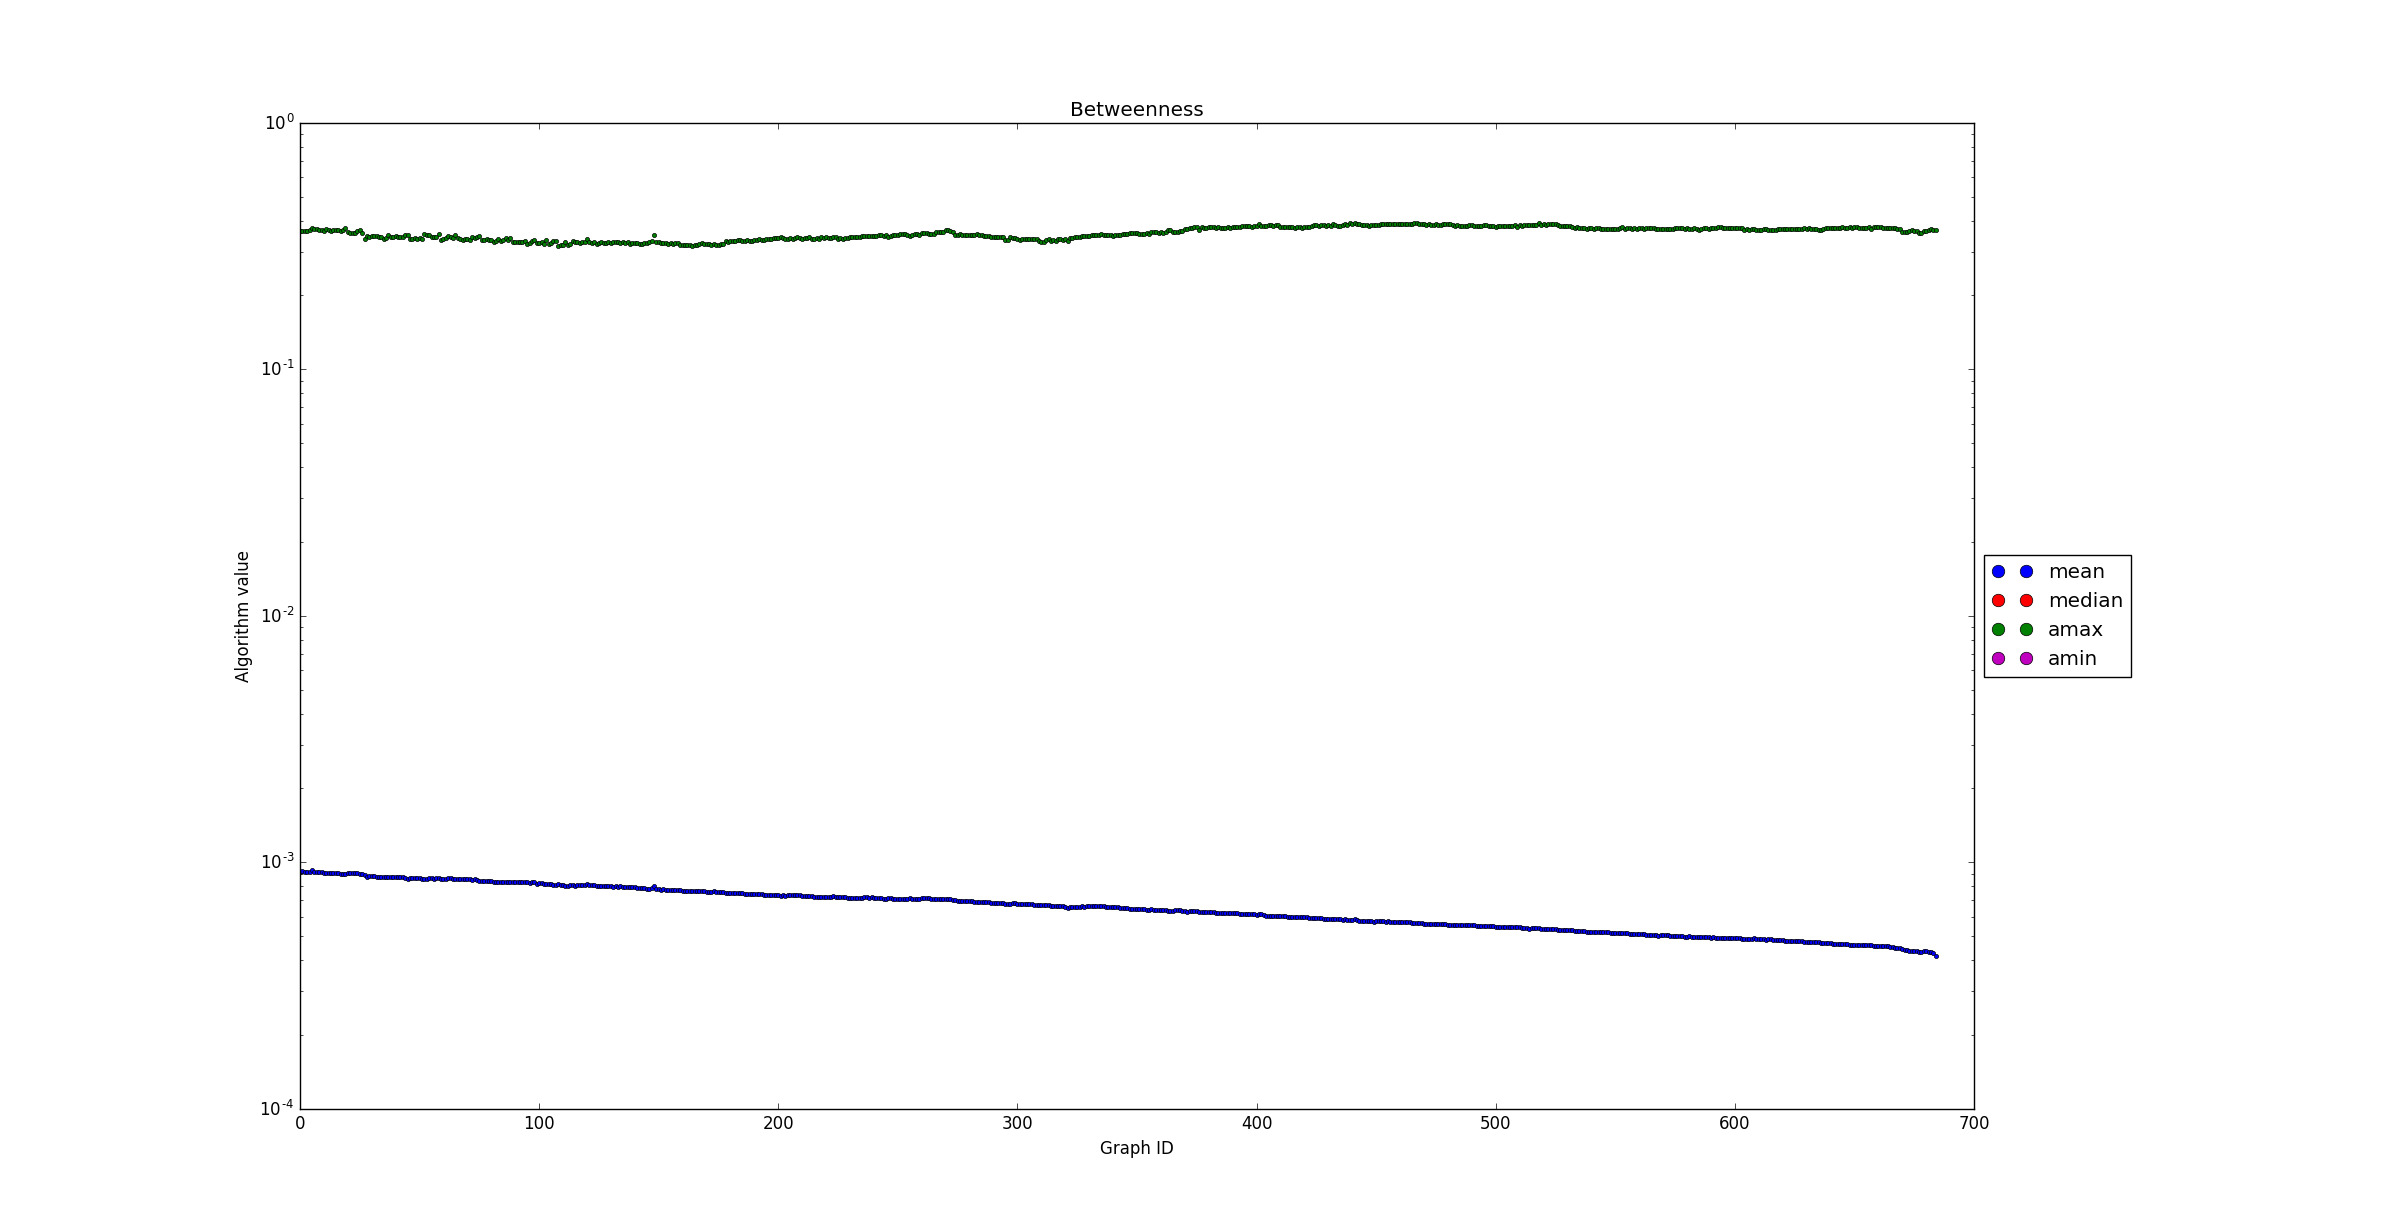
\includegraphics[width=\textwidth]{betweenness}
	\caption{Wyniki algorytmu betweenness}
\end{figure}
\FloatBarrier
\begin{figure}[h]
	\centering
	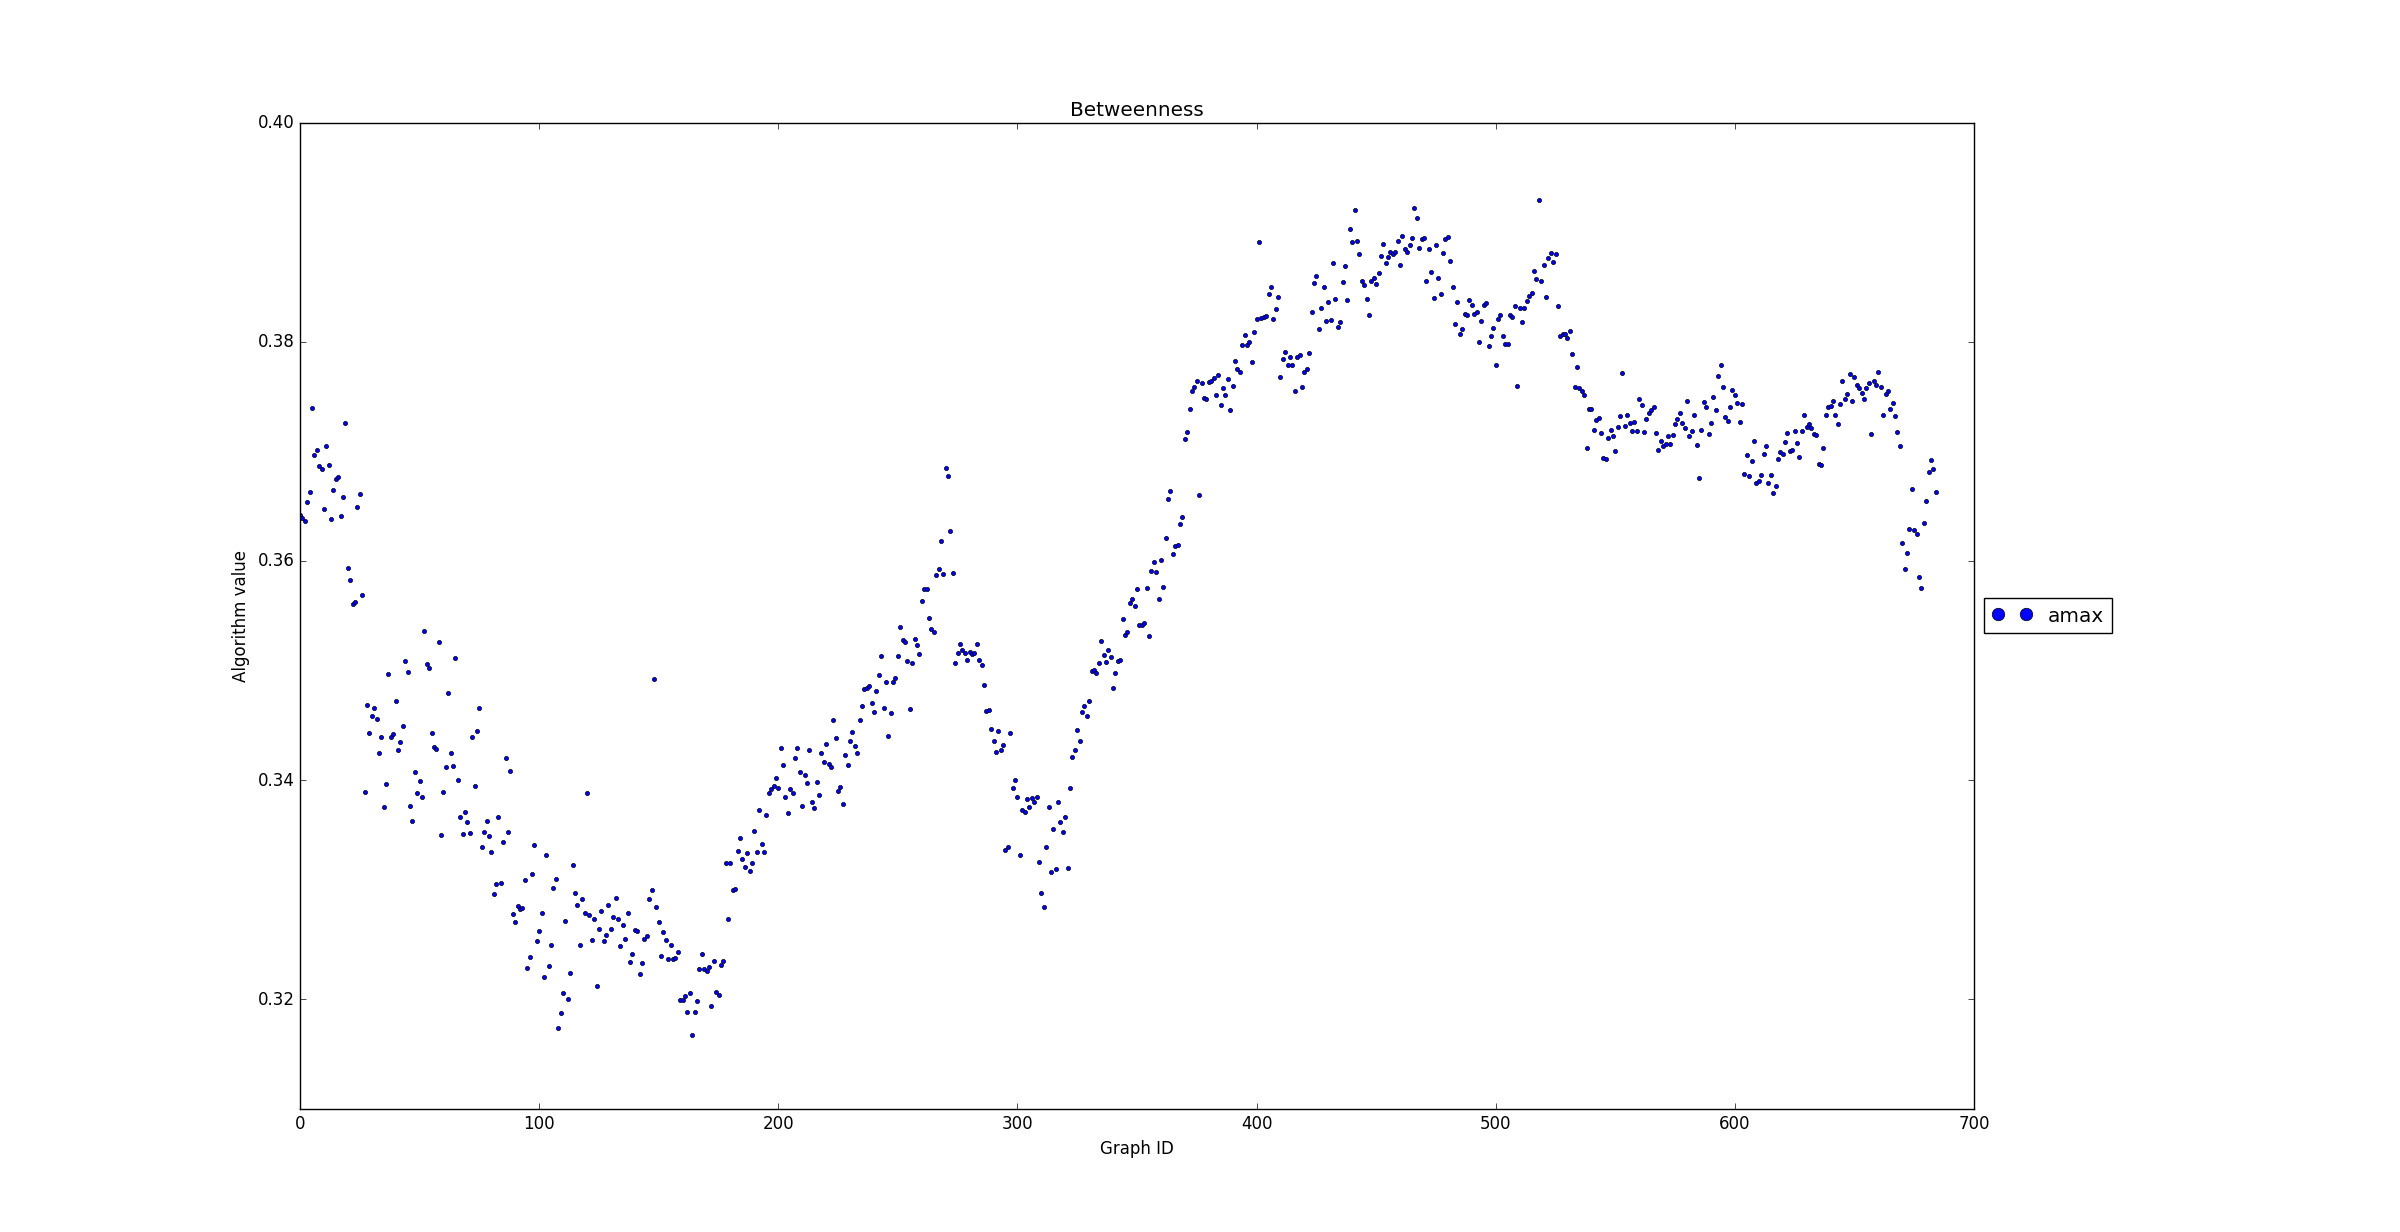
\includegraphics[width=\textwidth]{betweenness_max}
	\caption{Maksymalne wartości betweenness}
\end{figure}
\FloatBarrier
Niestałe zmiany maksymalnej wartości betweenness świadczą o tym, że struktura komunikacji w sieci zmieniała się dość znacznie. Im mniejsza jest różnica pomiędzy wartościami maksymalną i minimalną tym sieć jest bardziej równomierna w dostępie. Znaczy to że podczas dużego obciążenia jest mniejsze ryzyko, że większość ruchu będzie przechodziła przez jeden bądź kilka węzłów. Zmniejsza to prawdopodobieństwo awarii lub braku odpowiedzi.
\FloatBarrier
\begin{figure}[h]
	\centering
	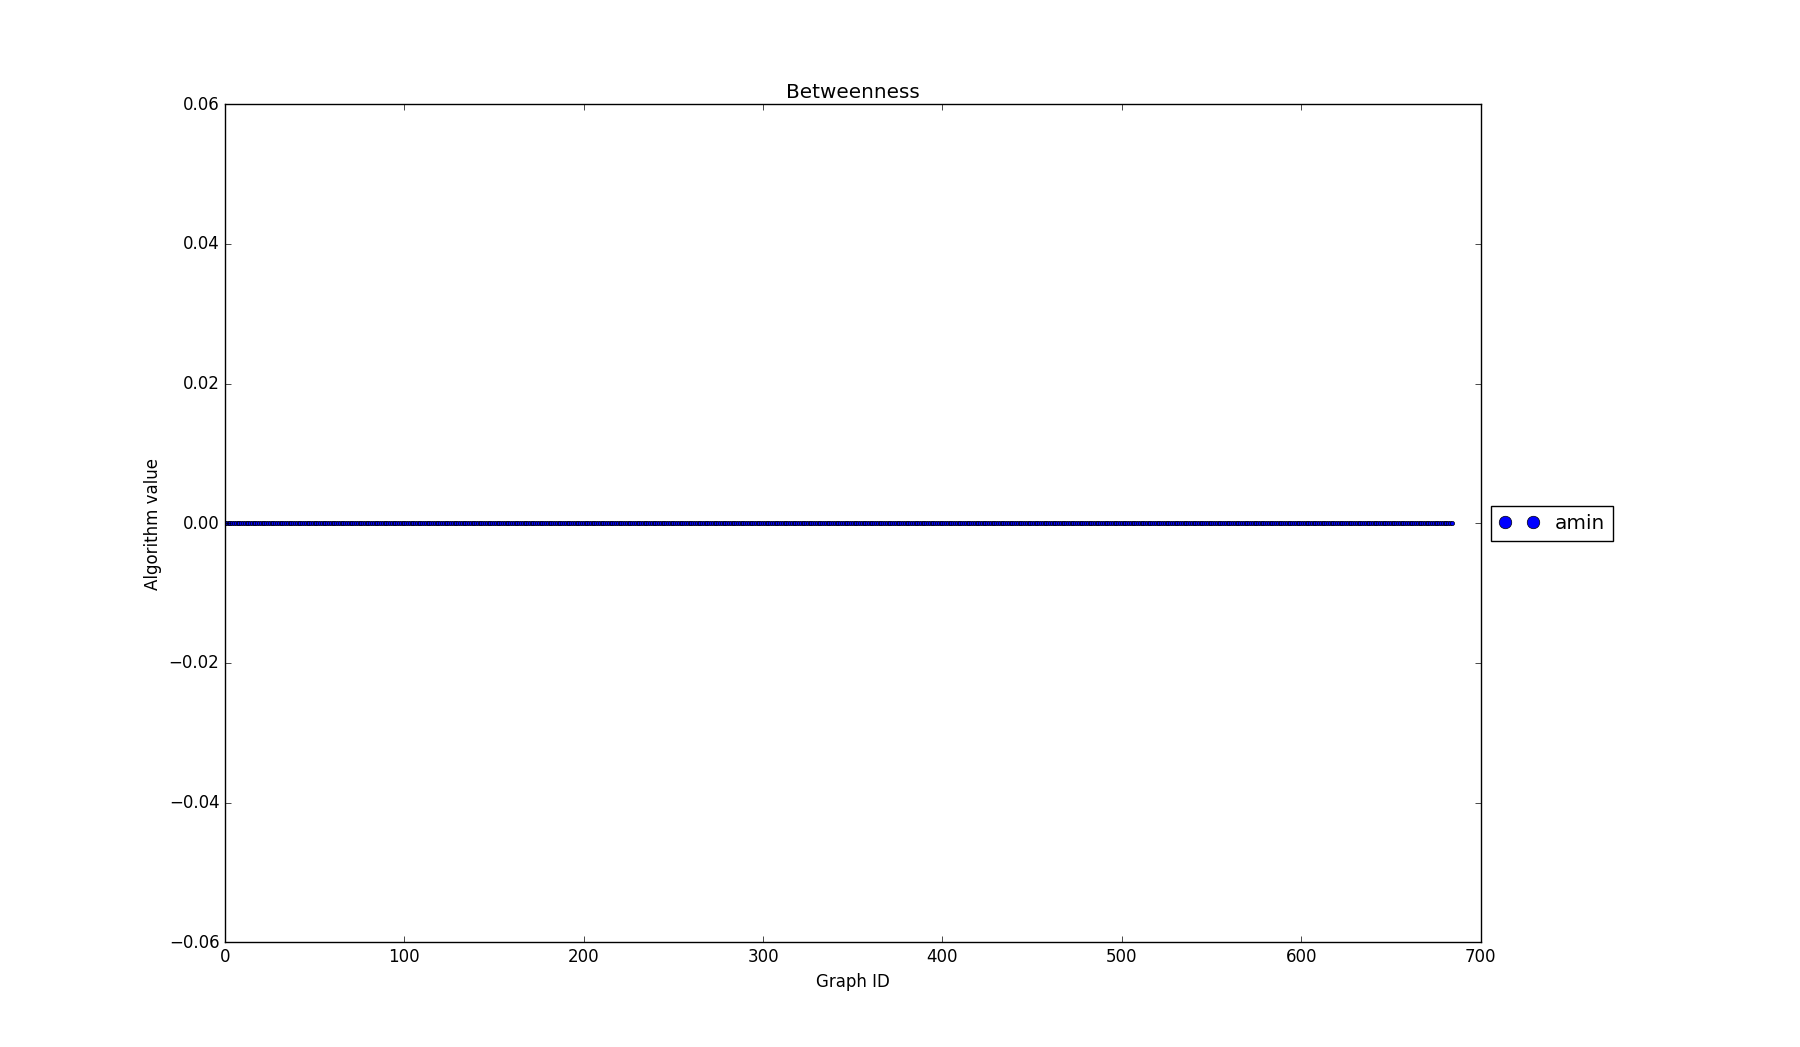
\includegraphics[width=\textwidth]{betweenness_min}
	\caption{Minimalne wartości betweenness}
\end{figure}
\FloatBarrier\FloatBarrier
\begin{figure}[h]
	\centering
	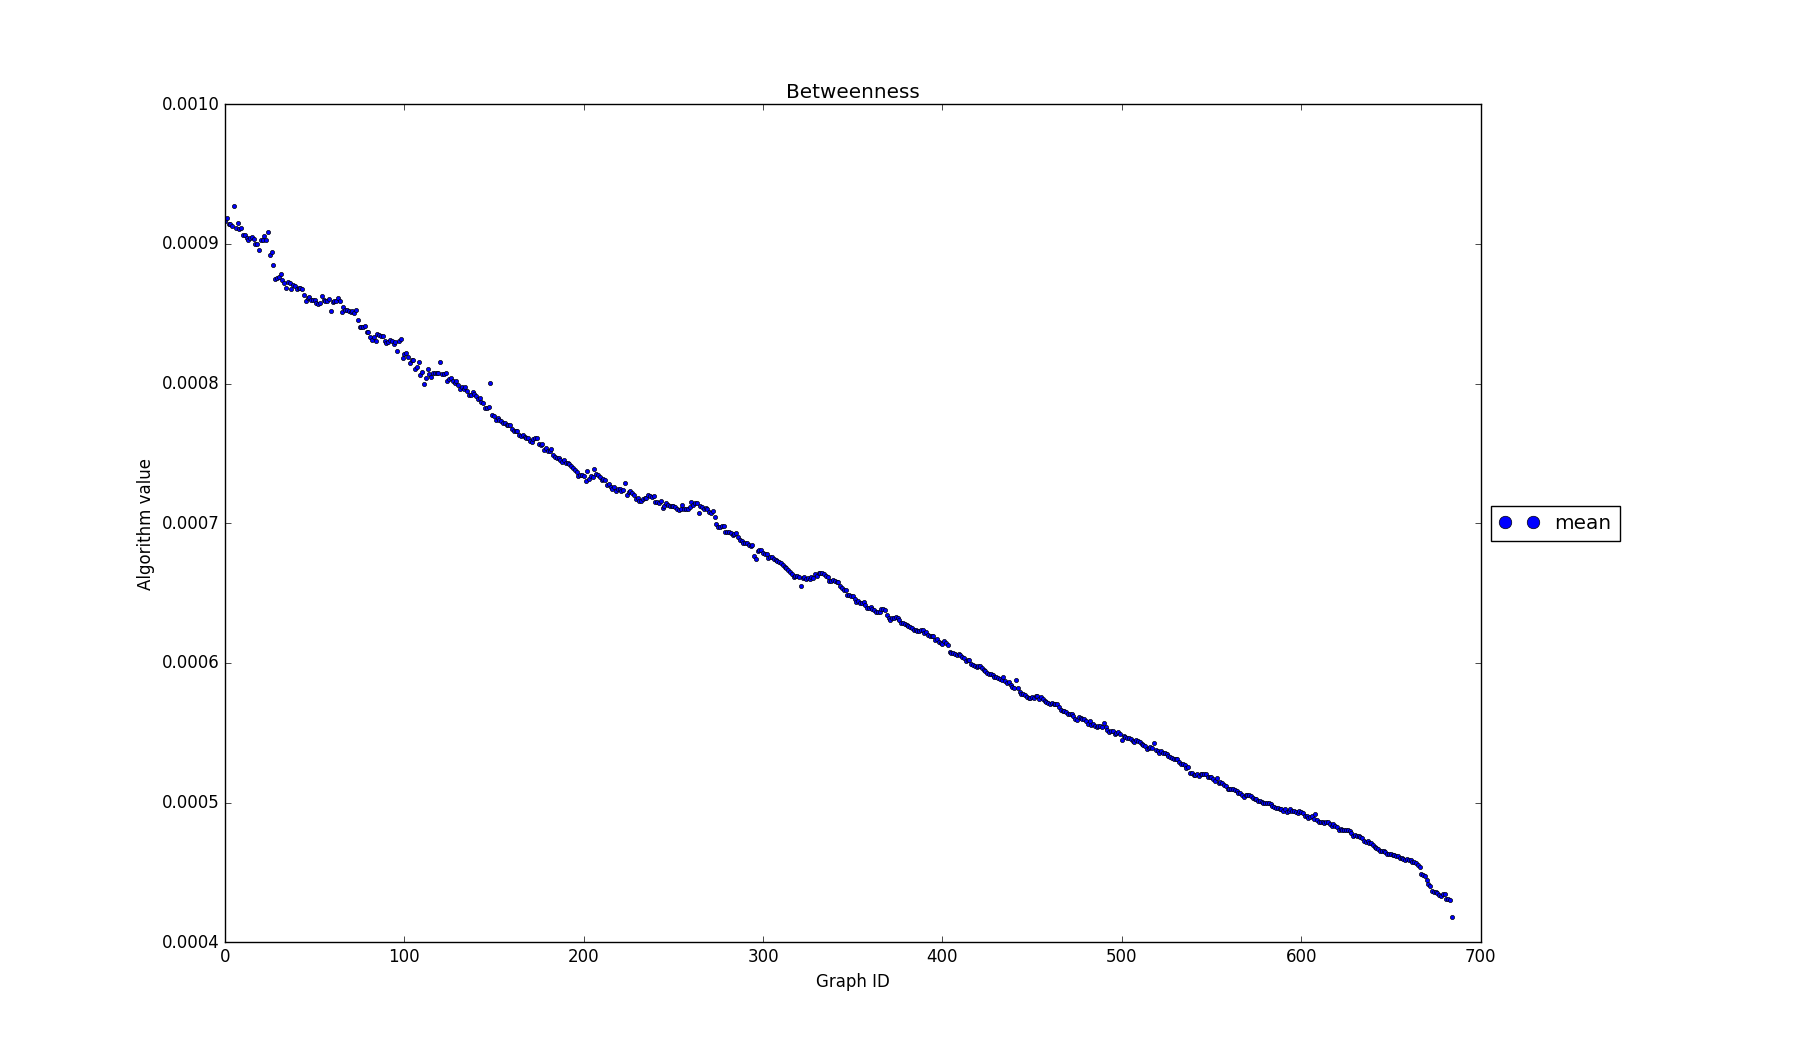
\includegraphics[width=\textwidth]{betweenness_mean}
	\caption{Średnie wartości betweenness}
\end{figure}
\FloatBarrier
Średnia wartość algorytmu spada w czasie. Jest to spowodowane głównie tym, że ilość wierzchołków w grafie rośnie a ich średni stopień maleje.
\FloatBarrier
\begin{figure}[h]
	\centering
	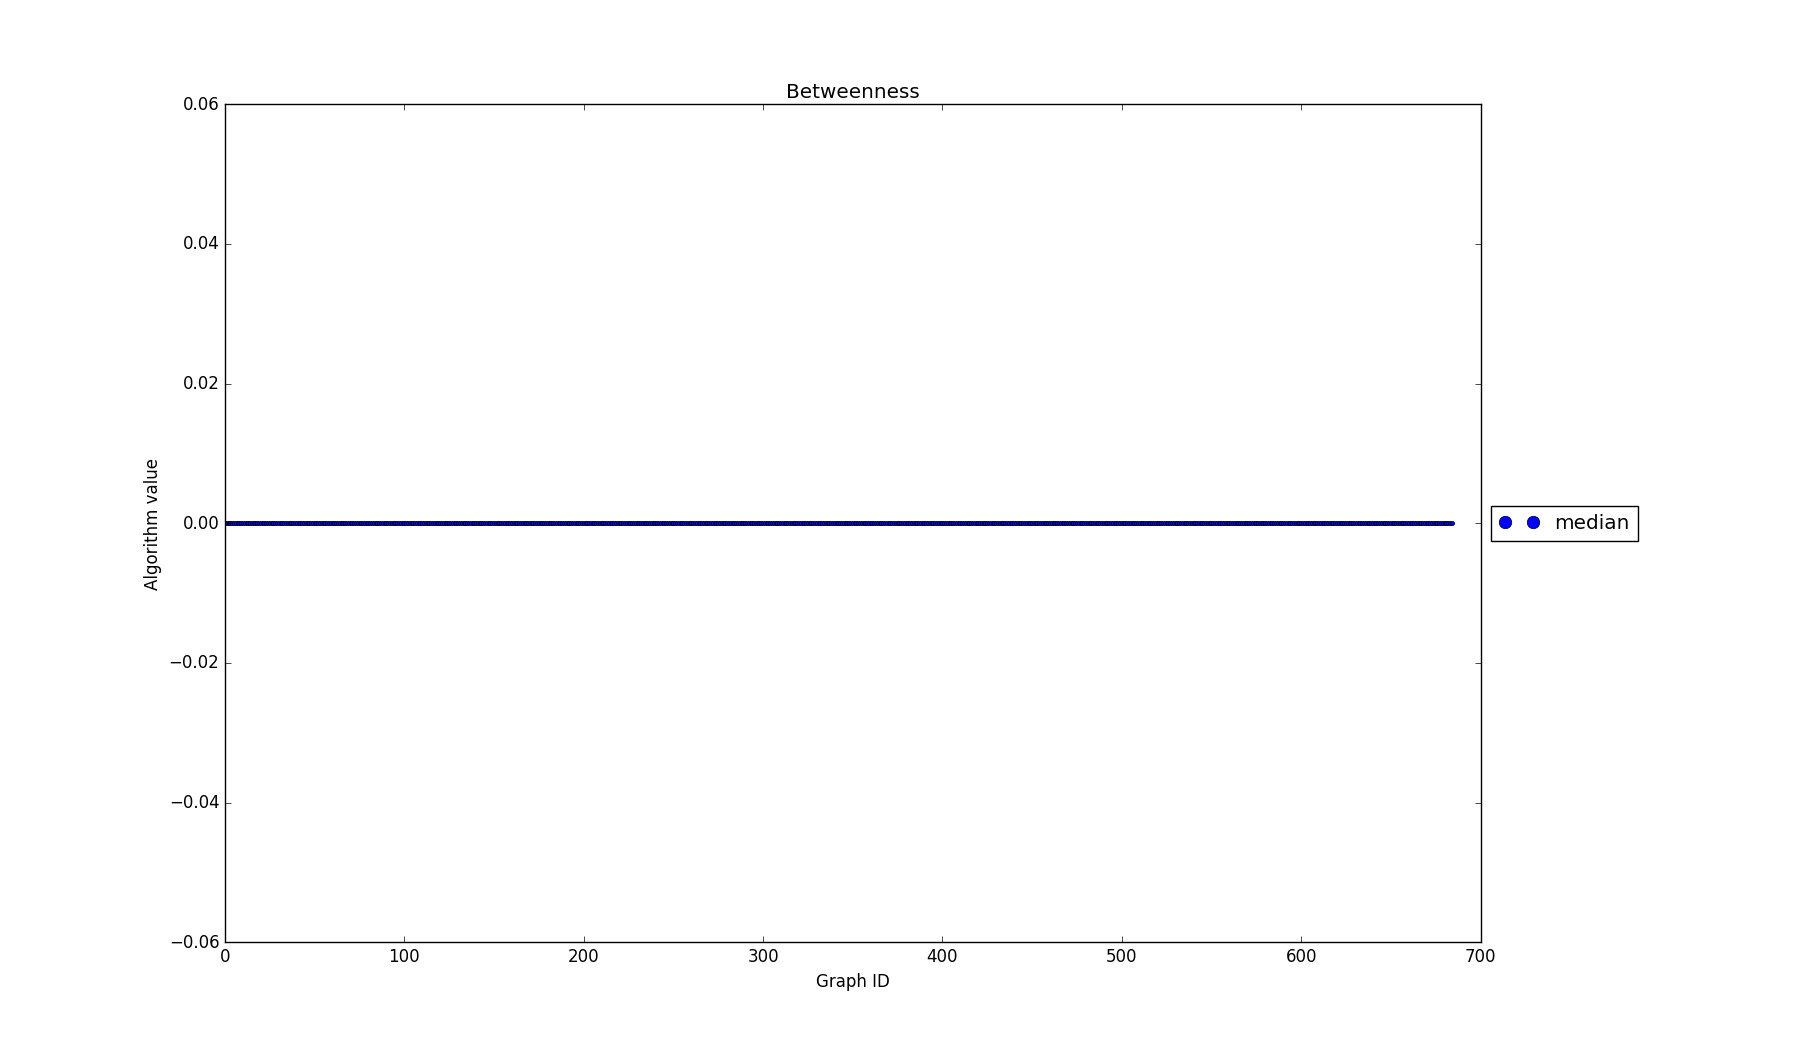
\includegraphics[width=\textwidth]{betweenness_median}
	\caption{Mediana wartości betweenness}
\end{figure}
\FloatBarrier
\newpage